We evaluated our technique in phases. First, we generated fake data that validates the correctness of the model, then we evaluated a small portion of the 
dataset, and finally evaluated on the full dataset.

\subsection{Generated Data}
The core algorithm relies on finding a $P$ and $Q$ matrix that relate users and businesses to latent factors (the columns of $P$ and $Q$). 
Figuring out specifically how a user (u) feels about a business(b) is just a matter of taking the dot product of $P_u$ and $Q_b$. 
Therefore, we started evaluation by randomly generating a $P$ and $Q$ matrix, and then creating the rating table based on the 
matrices. Running our algorithm on this data yielded similar $P$ and $Q$ matrices, which indicated that the algorithm was (fundamentally) doing what
we expected it to do.

\subsection{Real Data}
However, using generated data shows nothing about the validity of our model. In order to show just how effective our model would be, we needed to evaluate on the actual
businesses data from Yelp. We started evaluation by taking dense chunks of data from the Yelp set. Thus, we'd only have a couple of thousand ratings (instead of hundreds of thousands). 
This step was critical to expose inefficiencies in our calculations (indeed, once we started doing this, we immediately realized the need to switch our code from Python to a C++ module).

For training, we removed California's businesses ratings from the Yelp data set. This meant removing roughly \numBusCA businesses from \numBusTotal total businesses and \numRatingCA from \numRatingTotal ratings. Figure~\ref{fig:nocal} shows a plot of RMSE vs. K for all data excluding California's. For the evaluation step, we ran our algorithm on ratings for California businesses only. Figure~\ref{fig:cal} for a plot of RMSE vs. K for ratings only on California businesses. No parameters were changed between the training and evaluation run. The graphs show that the K-values have roughly the same effect on RMSE in both cases. Thus, a K-value that gives a poor RMSE value in the data excluding California gives a good RMSE value in the data for California (and vice versa). This result indicates that our model works well on data which we did not train or tune with.

\begin{figure}[ht!]
	\centering
%%	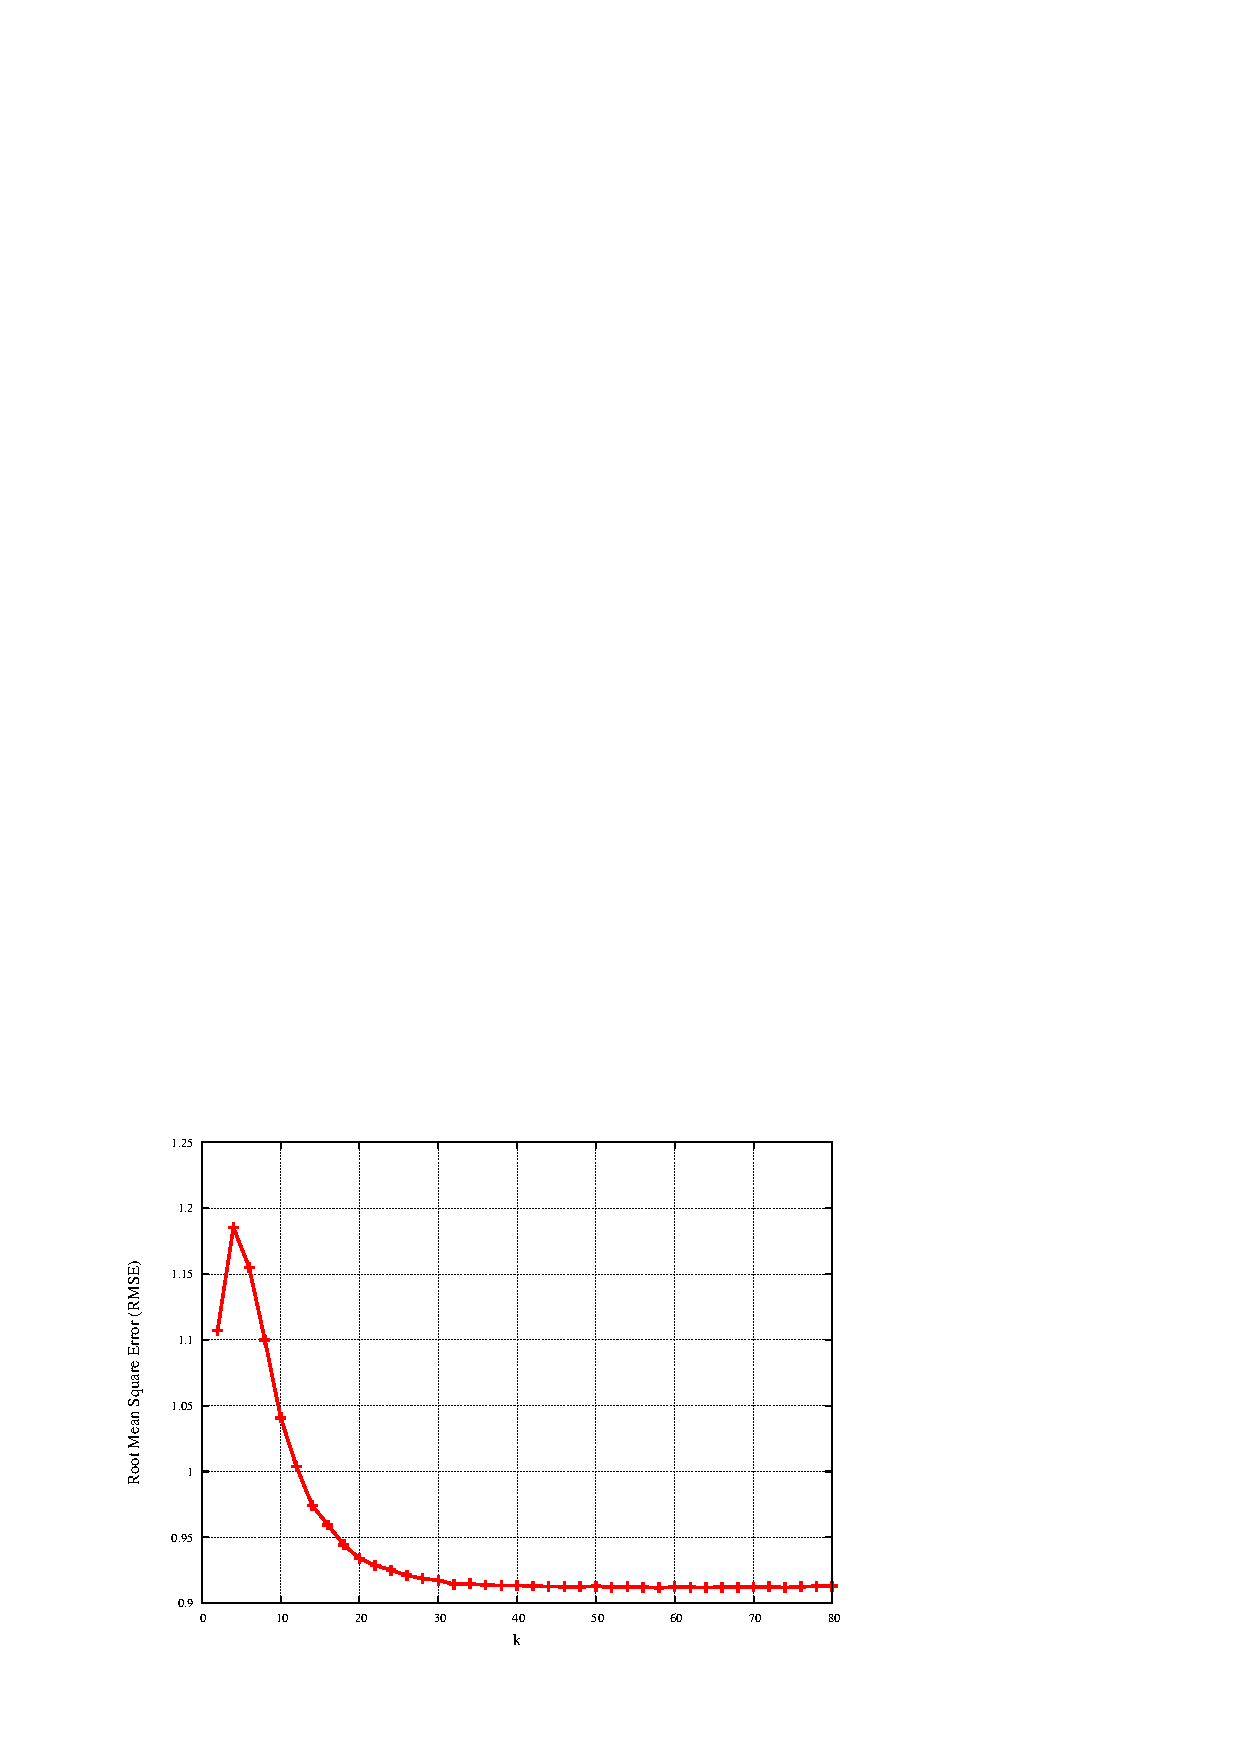
\includegraphics[scale=0.5]{figures/nocal.pdf}
	\caption[]{A plot of RMSE vs. K for all ratings excluding California businesses}
	\label{fig:nocal}
\end{figure}


\begin{figure}[ht!]
	\centering
	%%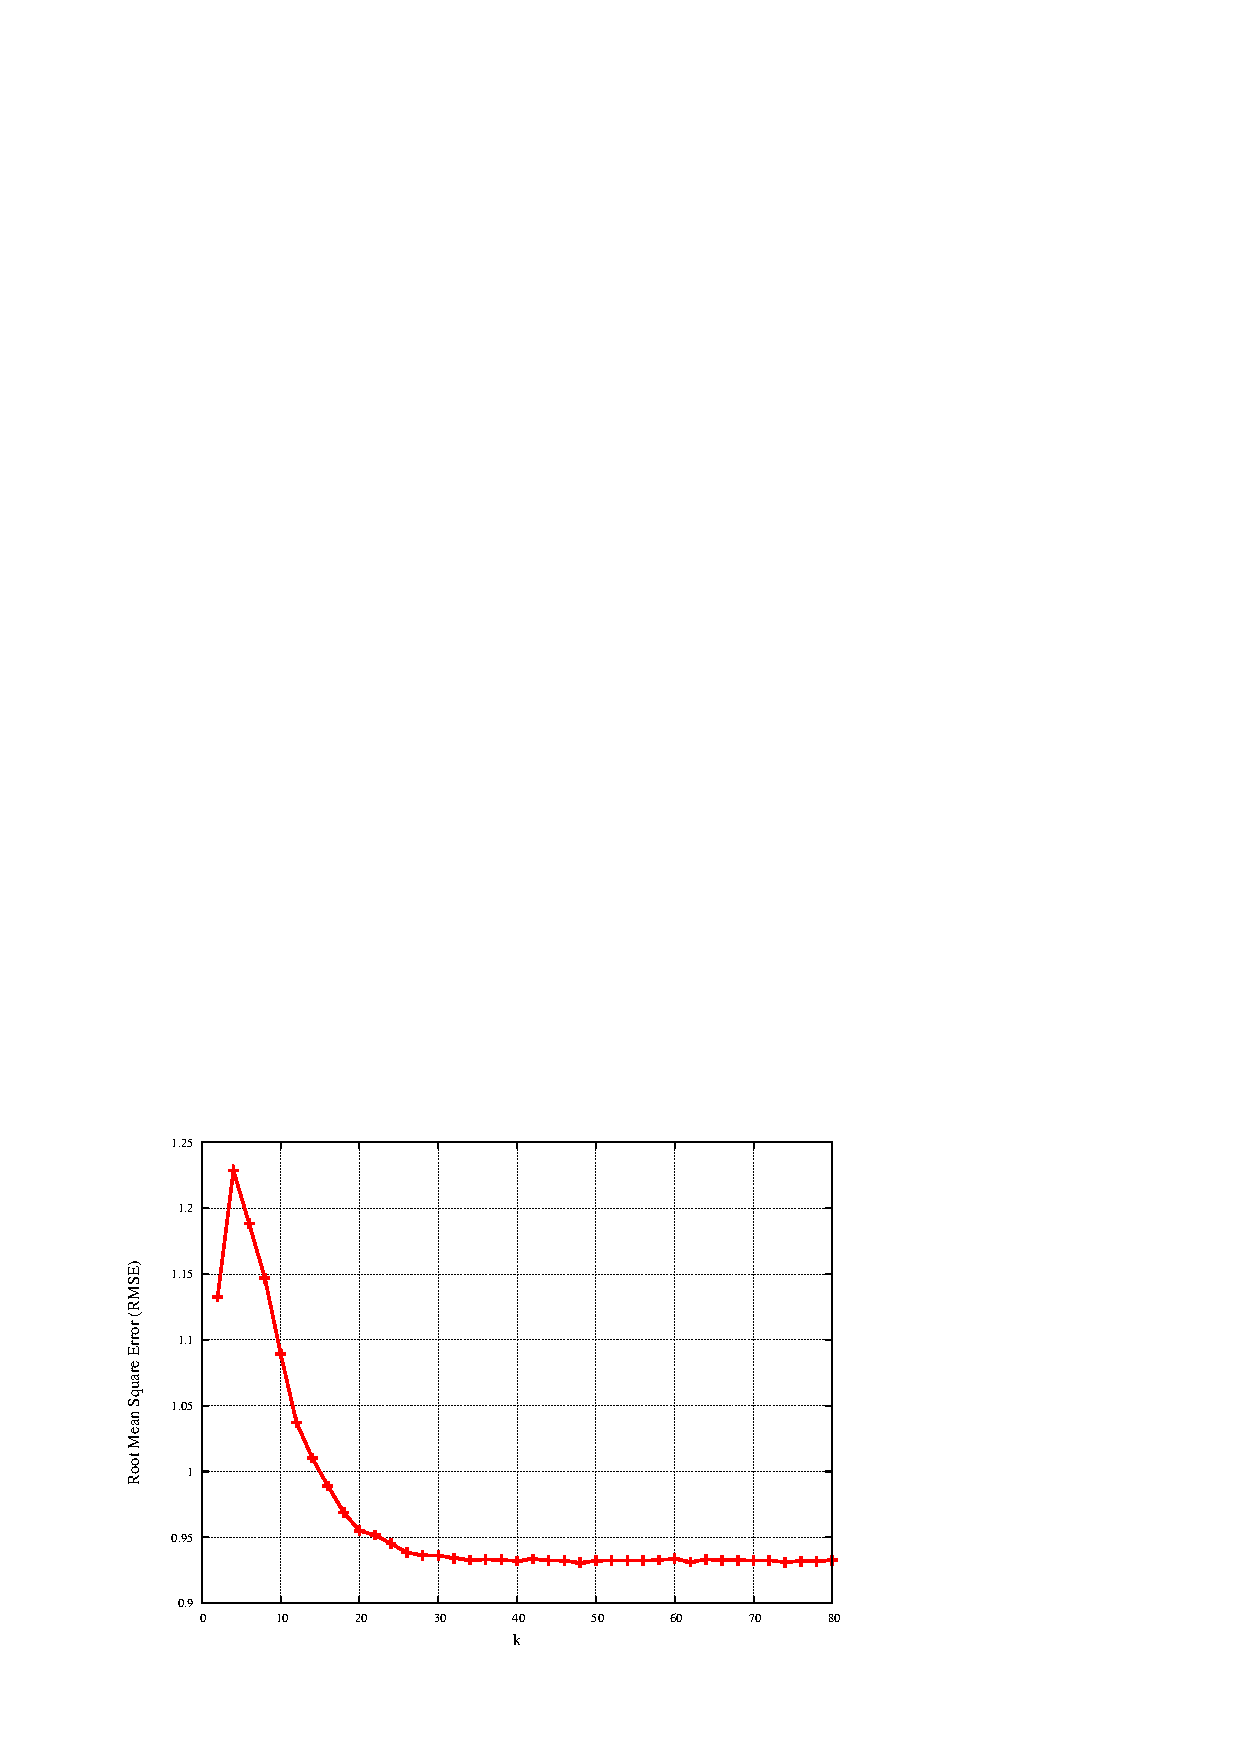
\includegraphics[scale=0.5]{figures/cal.pdf}
	\caption[]{A plot of RMSE vs. K for all ratings on California businesses}
	\label{fig:cal}
\end{figure}

\begin{figure}[ht!]
	\centering
	%%\includegraphics[scale=0.5]{figures/norm.pdf}
	\caption[]{A plot of RMSE vs. K for all ratings excluding California businesses without normalization}
	\label{fig:norm}
\end{figure}

We also evaluated the effect of normalization by running the same tests as above on businesses excluding California with and without a normalization factor. Figure~\ref{fig:norm} shows a plot of the same ratings and businesses as Figure~\ref{fig:nocal} without normalization.

\subsection{Interpreting Results}
As we increase the K-values, the RMSE value approaches a minimum value which it rarely dips below. For us, we were able to achieve an RMSE of \bestRMSE when K=\bestK. Increasing K beyond this did not improve RMSE, and would even cause over-fitting. What's particularly interesting about our result is that it shows predictions across a wide variety of businesses-genres can be useful in predicting interests in unrelated genres. For example, predictions for clothing shops can be used to help predict where you might like to go out to eat. We initially thought that using unrelated businesses to predict one another would yield to inaccurate results. However, when we excluded non-food related ratings from the dataset, we achieved worse RMSE results. See Figure~\ref{fig:foodnoly} for a plot.

We also compared our results to the winners of the Netflix prize, \cite{netprize}. Unlike our technique, the winners of the Netflix prize used a combination of different predictors working in unison to build a prediction engine. Ideally, we would build additional prediction engines to supplement ours. However, we were not able to do this due to time constraints. Overall, the winners of the Netflix prize achieved an RMSE value of \bestNetflixRMSE, which is roughly ~0.05 from our best RMSE of \bestRMSE. The difference between the accuracy of our results and the Netflix results is likely due to the fact that movies are much more controlled than businesses. Businesses are effected by location, price, quality of service, and hours of operation. Movies are always available and are displayed in a roughly uniform way. 

